%% This is an example first chapter.  You should put chapter/appendix that you
%% write into a separate file, and add a line \include{yourfilename} to
%% main.tex, where `yourfilename.tex' is the name of the chapter/appendix file.
%% You can process specific files by typing their names in at the 
%% \files=
%% prompt when you run the file main.tex through LaTeX.

\singlespacing{

\chapter{Software Workflows for Digital Materials}\label{chap:CAD}

\begin{figure}
  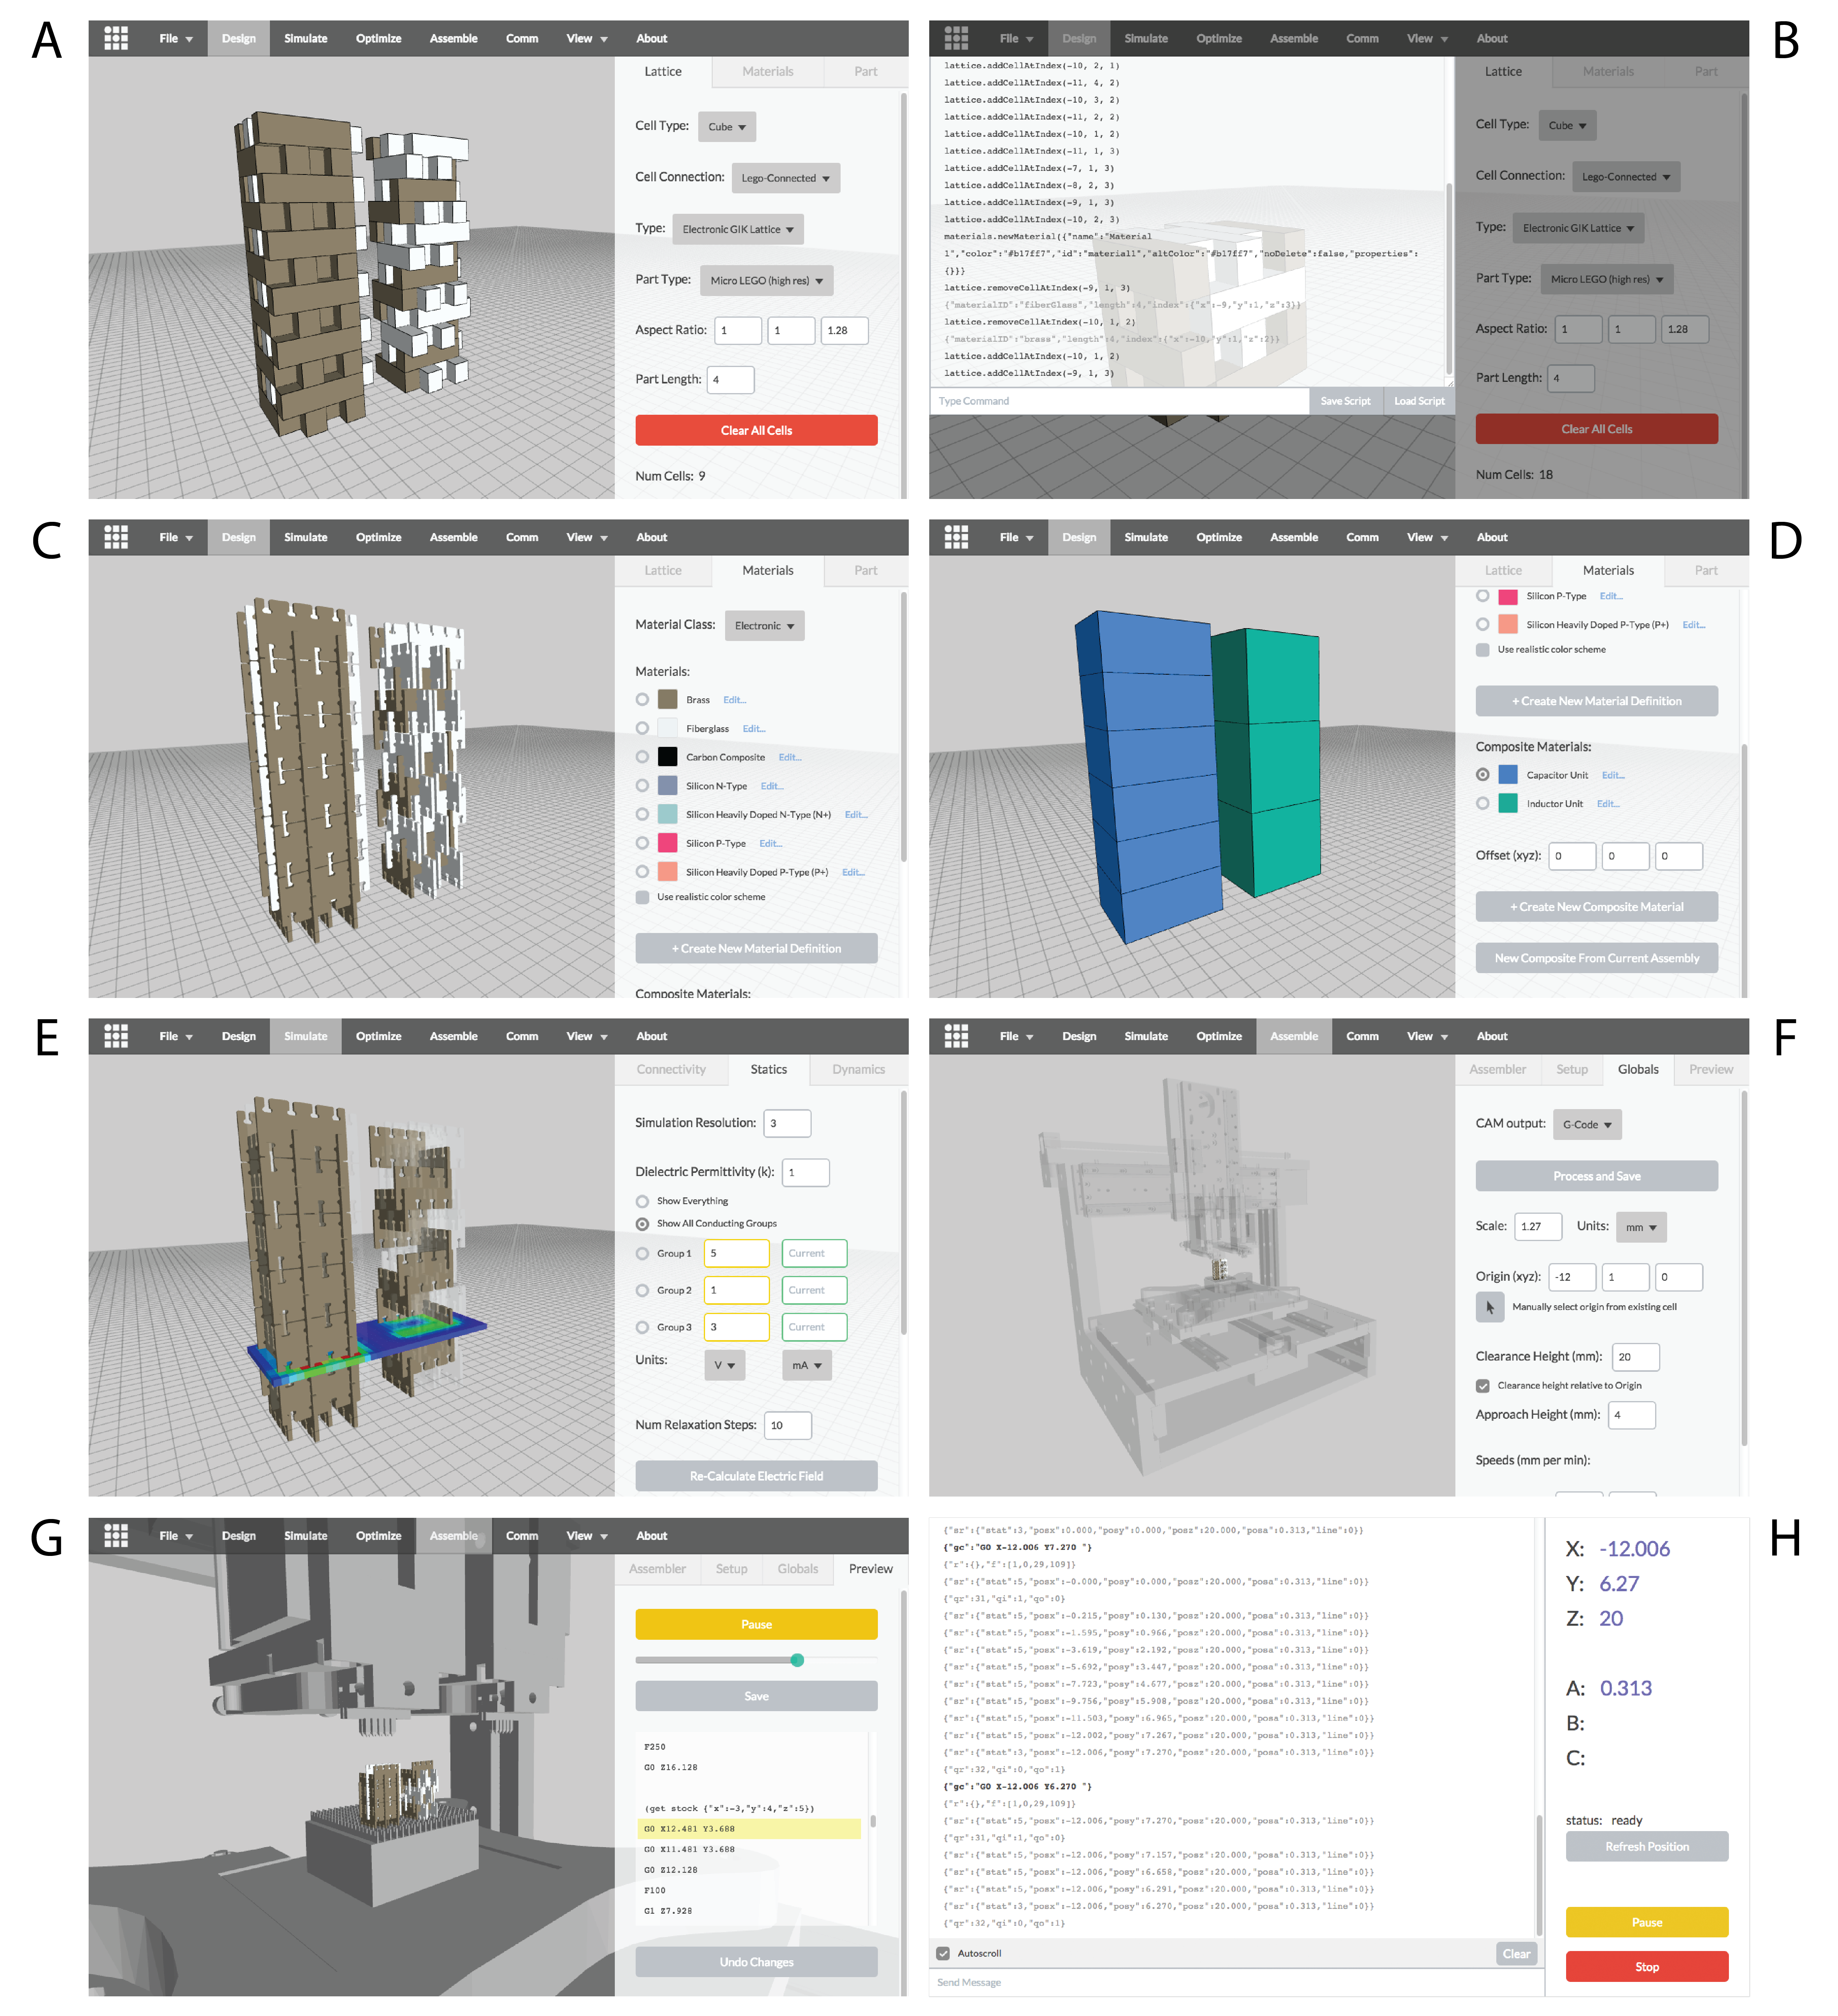
\includegraphics[width=\linewidth]{20151215DMDesignscreenshotsx8.png}
  \caption{Screenshots of DMDesign, a CAD / Simulation / CAM software package for digital materials. Structures are designed from multiple materials in a hierarchical \textbf{(D)}, 3D CAD interface or scripting API \textbf{(B)} that toggles between a "cell" and "parts" design representation \textbf{(A, C)}.  Simulation tools include mapping the potential field around arbitrary configurations of conducting and insulating parts \textbf{(E)}. CAM interface includes path planning and visualization of the assembly process \textbf{(F, G)} and serial interface with machine \textbf{(H)}.}
  \label{fig: designAssemblyGUIWide}
\end{figure}

\href{http://dma.cba.mit.edu/dmdesign/}{DMDesign} is a CAD/Simulation/CAM environment for digital materials that supports the current research efforts into part and assembler design at CBA.  In DMDesign, users construct multimaterial lattice assemblies in a virtual 3D environment, simulate their physical properties, plan out an assembly process, and communicate in realtime with assemblers to physically realize the design \cite{LangfordWillGhassaeiAmandaGershenfeld2016}.   A graphical overview of these capabilities is shown in Figure \ref{fig: designAssemblyGUIWide}.\\

DMDesign was built to simplify the process of designing and manufacturing digital material assemblies across a range of scales, application spaces, lattice topologies, and assembly processes. This chapter introduces some of the design principles behind DMDesign, namely, how abstraction is used to support a diversity of forms and functions.

\section{Design Abstraction}

\begin{figure}
  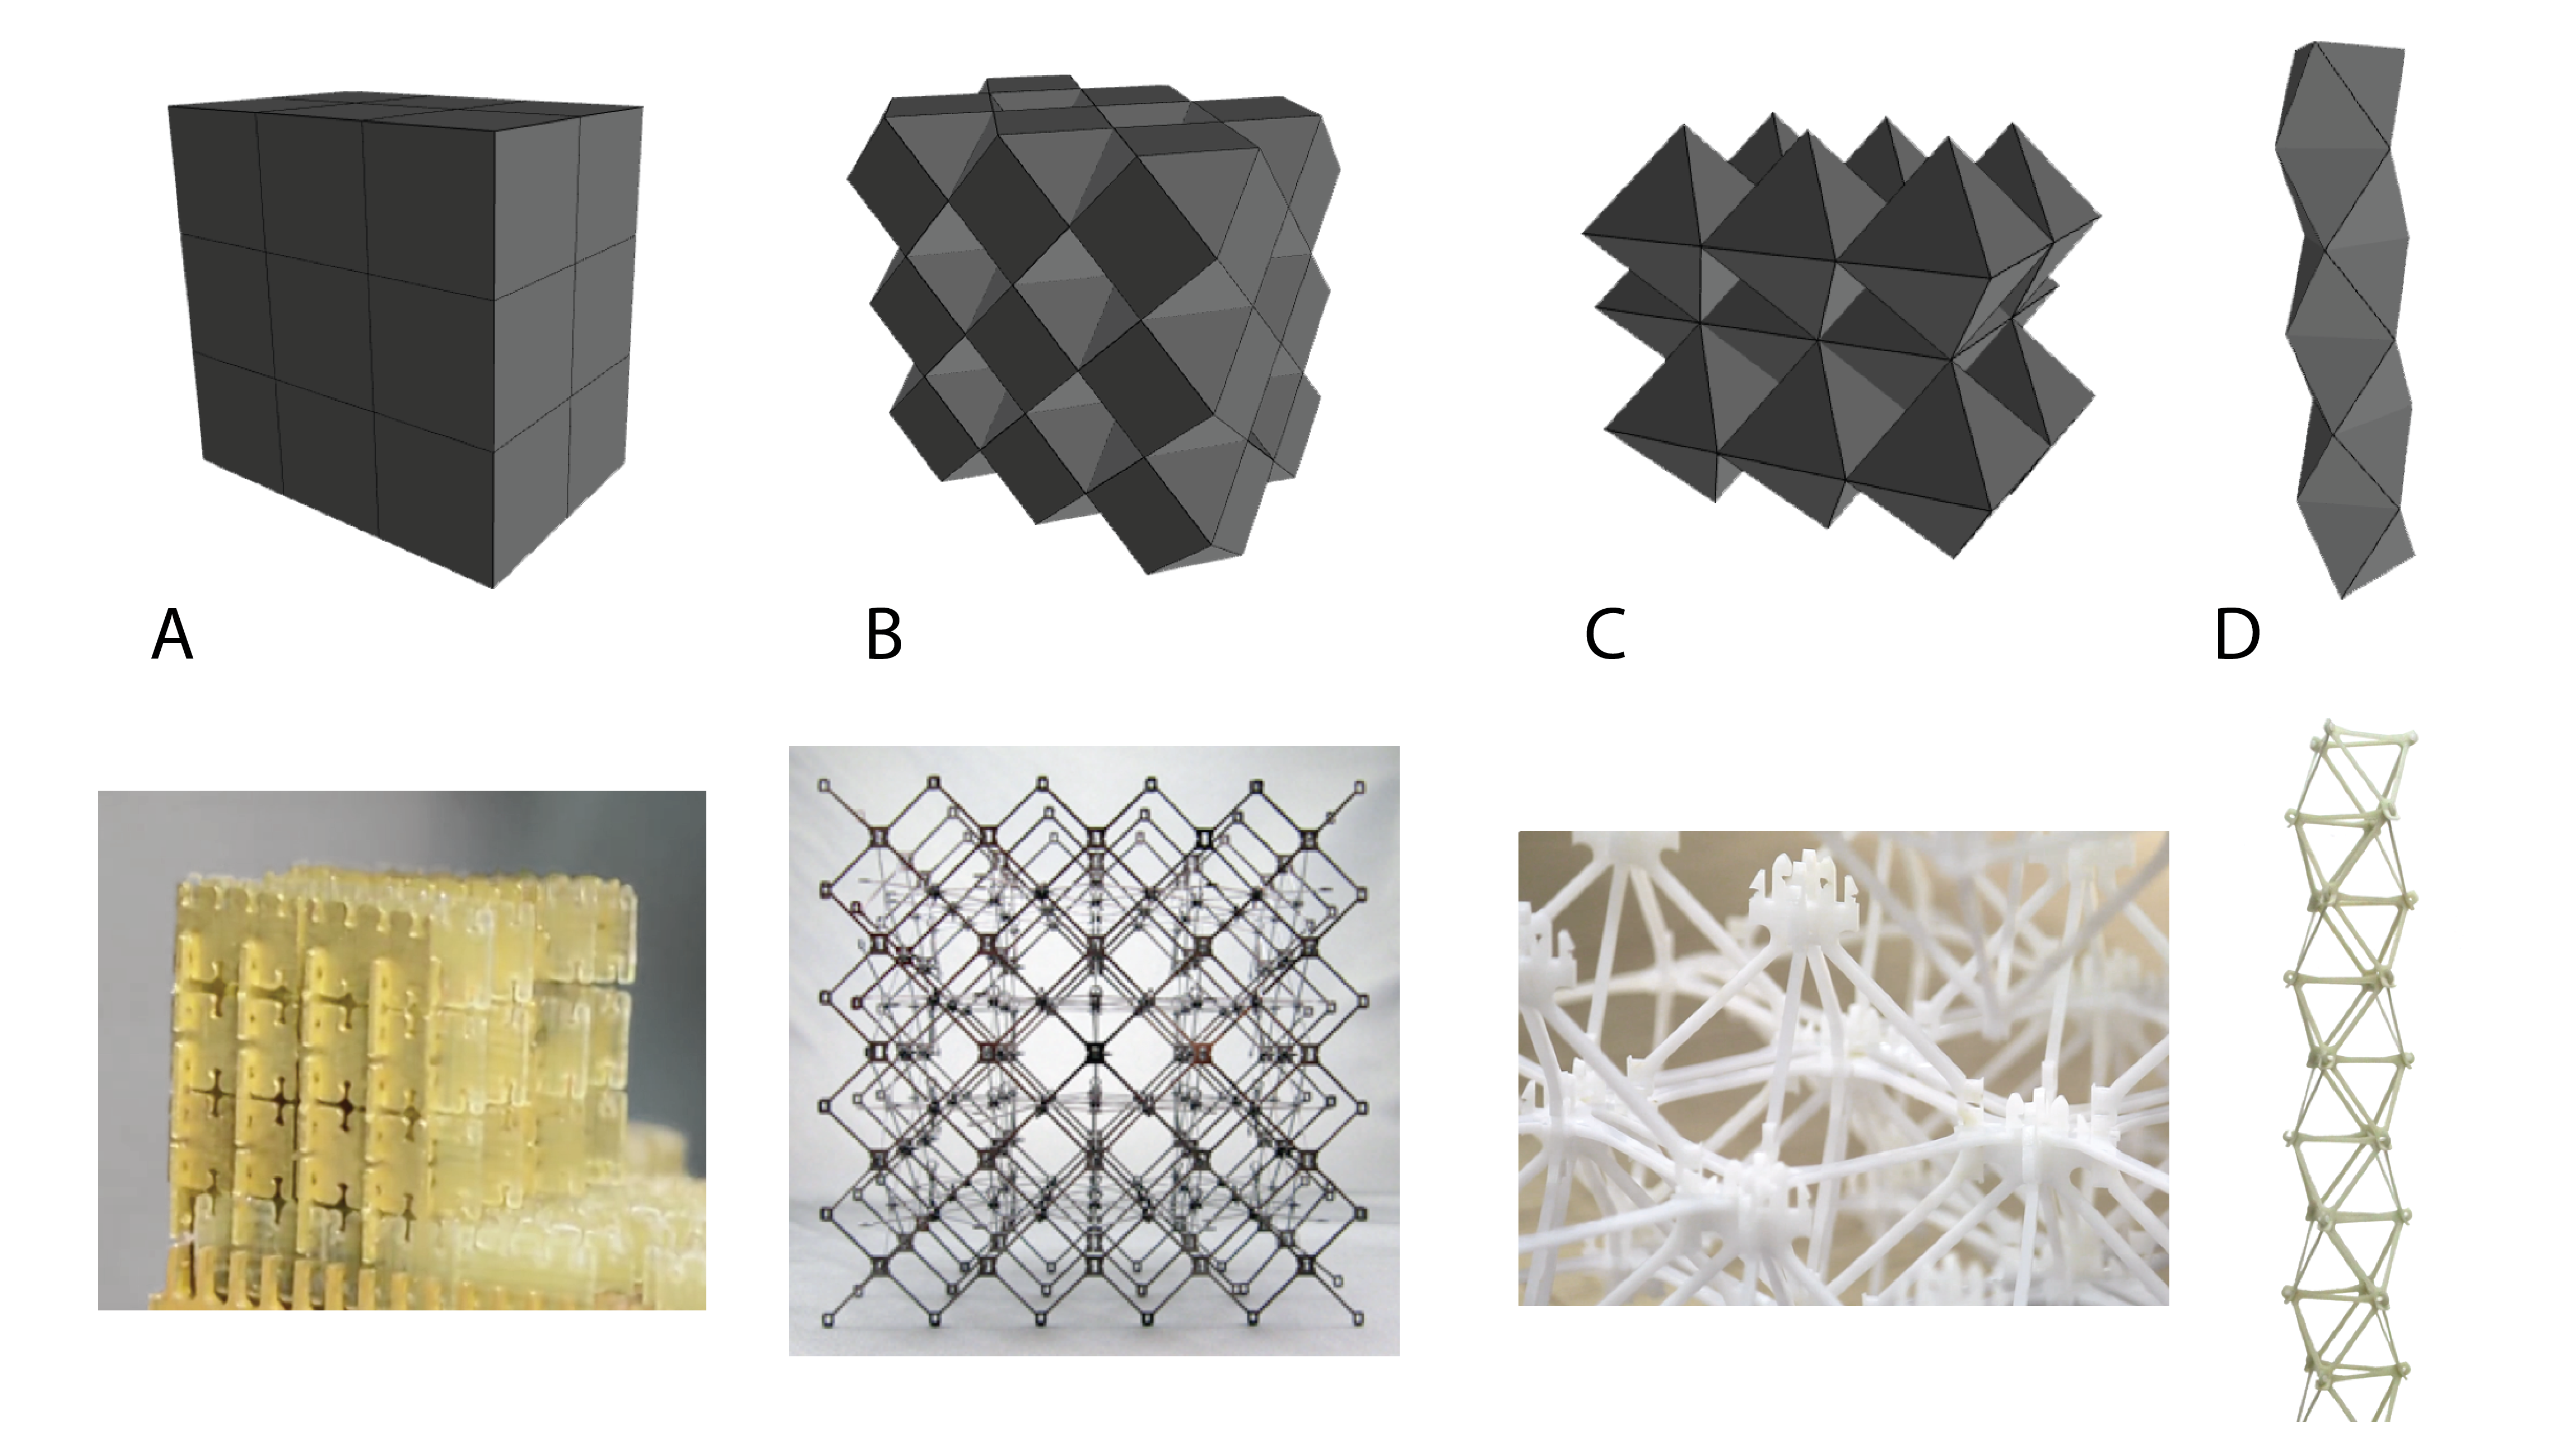
\includegraphics[width=\linewidth]{MechanicalLattices.png}
  \caption{A variety of lattice geometries and their corresponding digital material assemblies.  From left to right: cubic lattice with electronic GIK assembly \textbf{(A)}, cuboctahedron lattice with carbon-fiber composite assembly \textbf{(B)}, edge-connected octahedron lattice with laser cut delron voxel assembly \textbf{(C)}, face-connected octahedron lattice with injection molded glass-filled nylon truss \textbf{(D)}, and Kelvin lattice with electronic "phoxel" assembly \textbf{(E)}.}
  \label{fig:MechanicalLattices}
\end{figure}

As described in Chapter \ref{chapter:RelatedWork}, digital materials are discrete parts that interconnect to form a regular, periodic lattice.  Accordingly, the DMDesign internals assume an underlying discrete representation of geometry.  The core of the CAD interface prompts users to arrange cells into 3D lattice \textit{assemblies}.  The particular lattice topology used in the CAD workflow is application specific; several available lattice types are depicted in Figure \ref{fig:MechanicalLattices}.  At the time of writing this, a total of 11 different lattice topologies are supported in DMDesign.\\

\begin{figure}
  \includegraphics[width=\linewidth]{PartAbstraction.png}
  \caption{Abstraction of cell representation from physical part geometry.  In the "lego"-connected cubic lattice, cells are placed in an an assembly with no notion of the physical parts they represent.  For example, a cell could represent a piece of LEGO, an electronic GIK part, or even a single strand of DNA in a DNA Bricks assembly.  \textit{Image Credit: Will Langford (GIK Images), Ke et al. (DNA Bricks) \ref{Ke2012}}}
  \label{fig:PartAbstraction}
\end{figure}

The fundamental unit of geometry in DMDesign is a lattice cell, both in its outward facing CAD interface and its internal data representation.  This may seem strange since the assembly process happens at the granularity of a part, which may be different than a cell in terms of its geometry and connectivity on the lattice.  This abstraction was used to simplify the design interface and allow for a separation of the underlying geometrical representation of an assembly from its decomposition into parts.\\

Design abstraction maximizes portability of a single assembly definition across different processes and parts.  Figure \ref{fig:PartAbstraction} shows how a single lattice cell represents a variety of potential part types.  Different joining strategies may require breaking up the same underlying lattice geometry into different repeating units.  For example, a vertex-connected octahedron lattice may be broken up into interconnected X-shaped parts, square-shaped parts, or even 3D octahedral voxels.\\ 

Additionally, cells are a more useful unit of geometry as we move into simulation.  Parts that have been joined together to form a complete, constrained cell add rigidity to the structure.  In simulation we are typically concerned only with the behavior of these constrained, rigid elements of the lattice, as is the case for many high-performance aerospace applications.

\section{Design Hierarchy}

\begin{figure}
  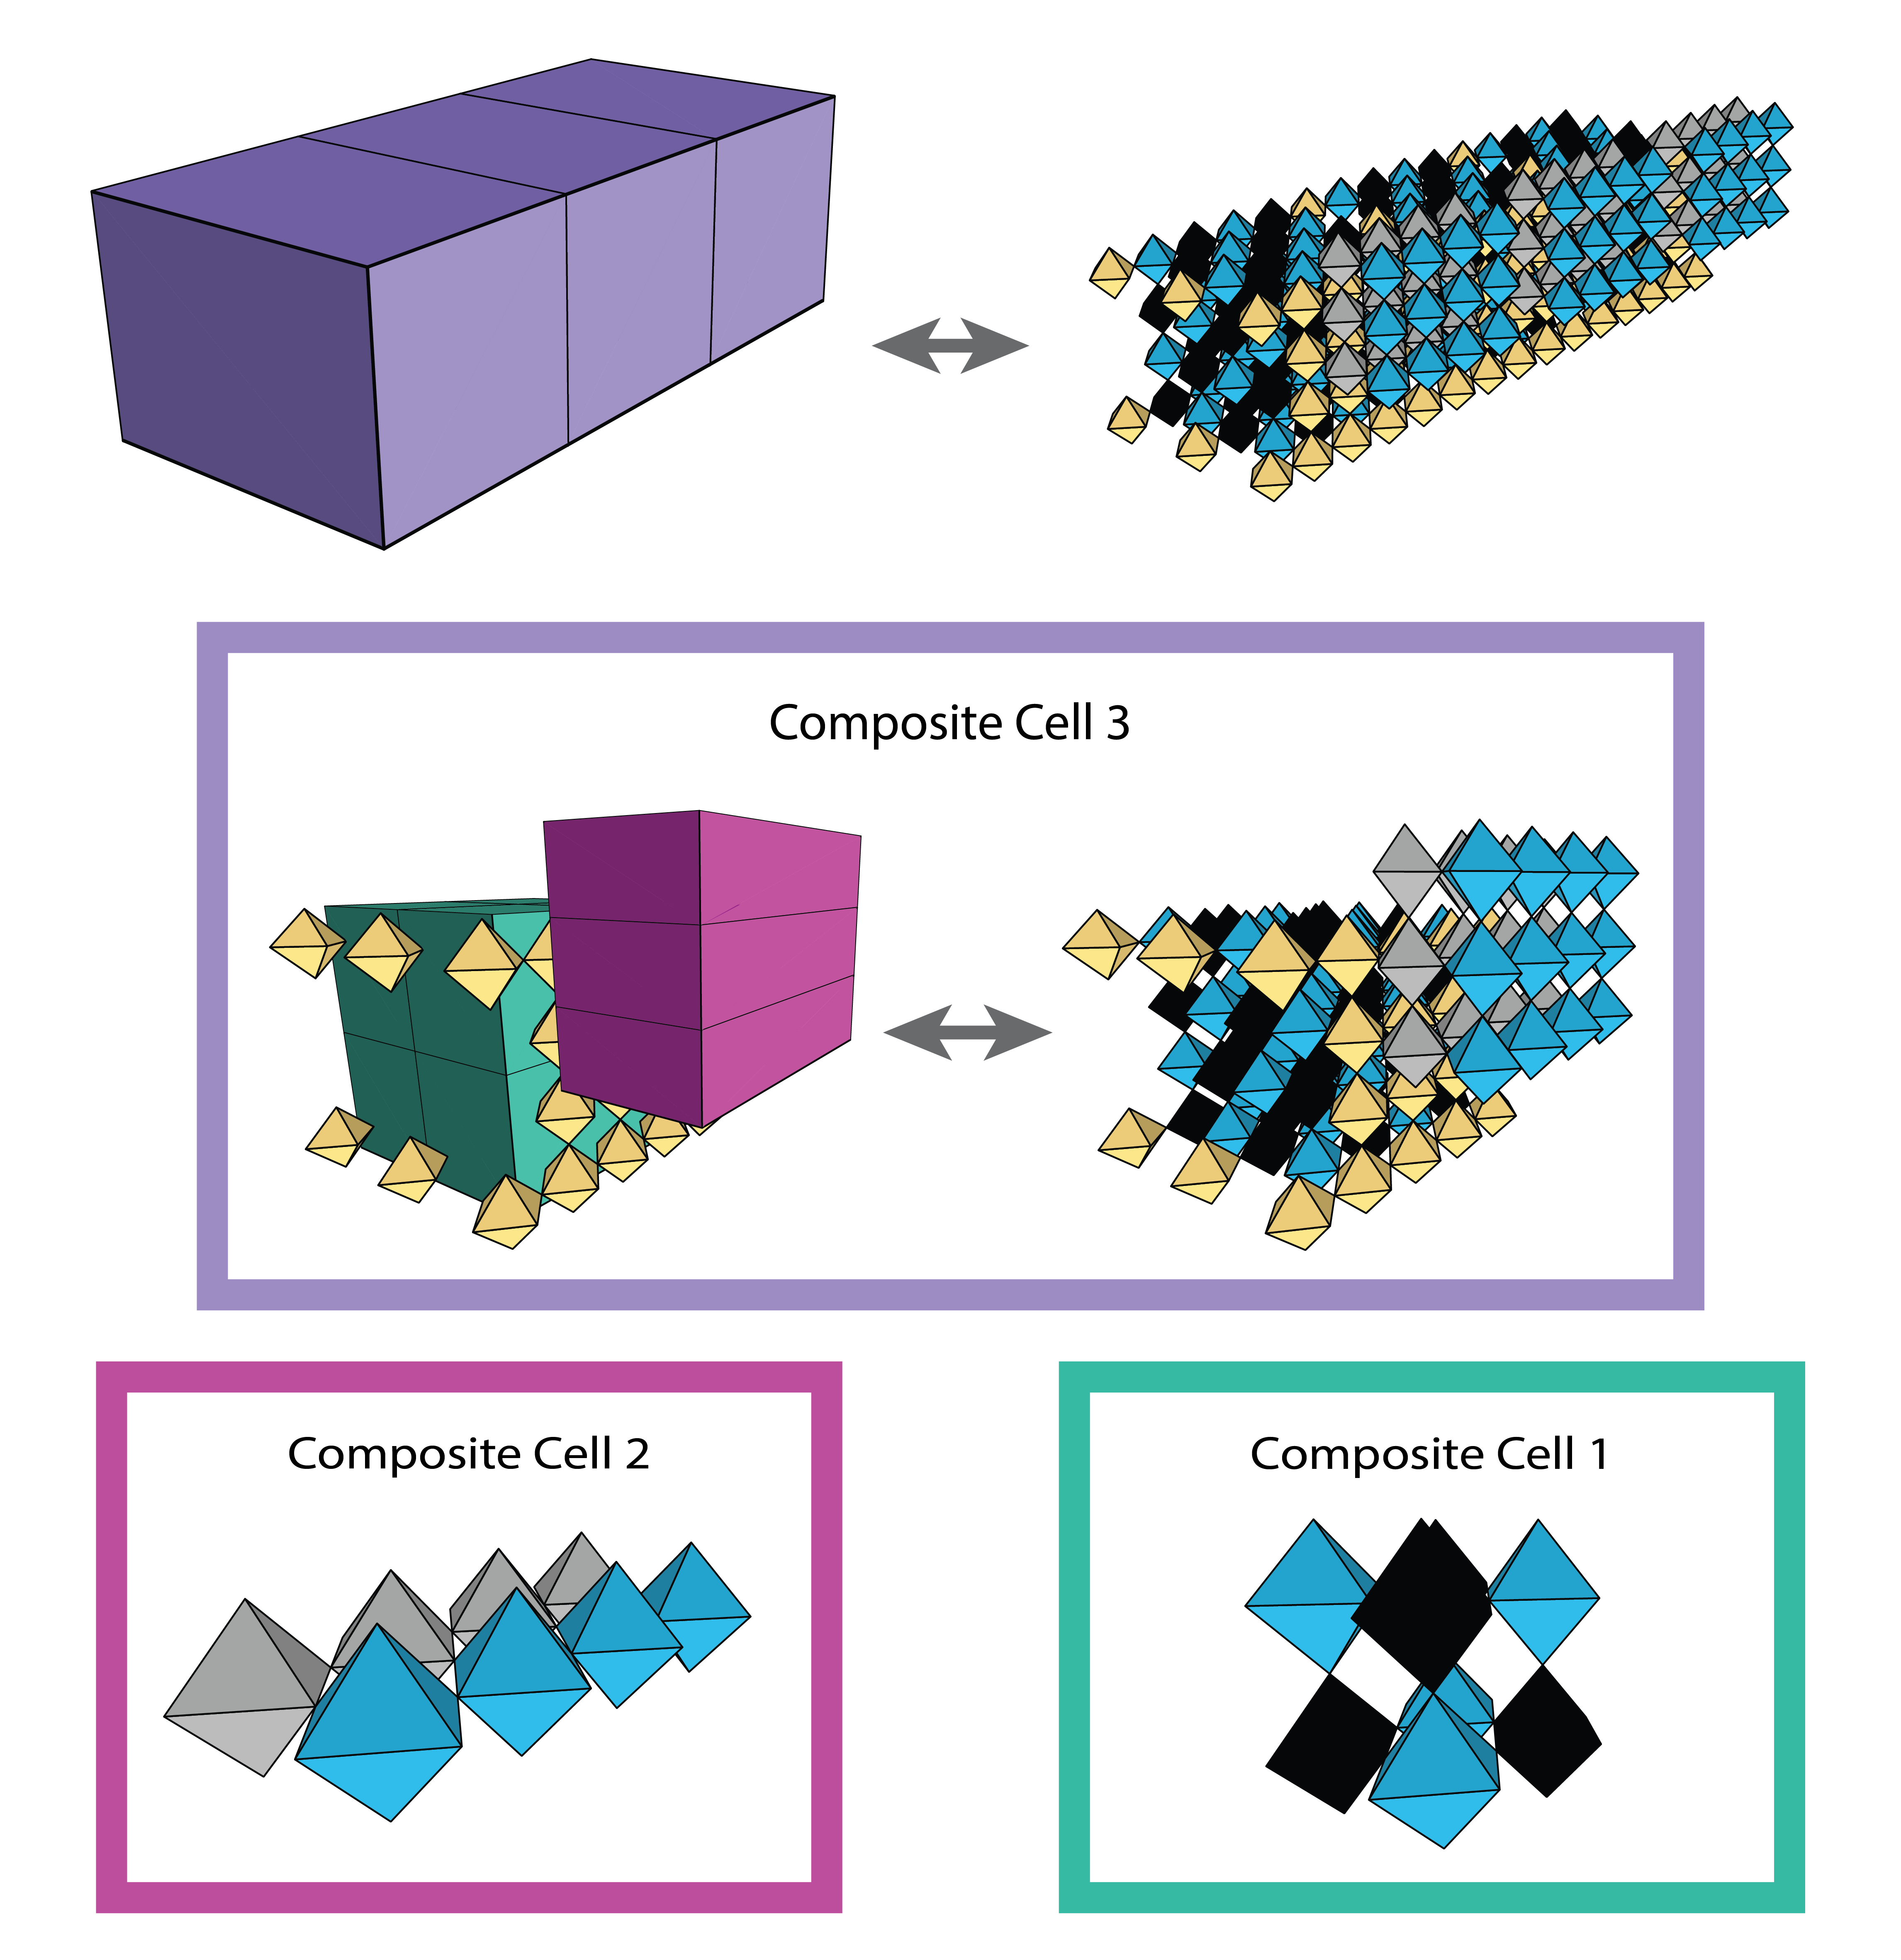
\includegraphics[width=\linewidth]{CompositeCells.png}
  \caption{Hierarchical assembly of a vertex-connected octahedron lattice.  Full assembly depicted in both hierarchical view and cell view (top, left and right).  Composite cell definitions 2 and 1 each contain two cell material types (bottom, left and right).  Composite cell definition 3 contains a mixture of composite cells and non-composite cells, depicted in both hierarchical view and cell view (middle, left and right).}
  \label{fig:CompositeCells}
\end{figure}

Design hierarchy is the establishment of parent/child relationships between elements of a design.  In the context of DMDesign, hierarchical data structures allow for a more sparse description of assemblies that contain many similar regions.  Hierarchical structures within DMDesign are called "composite cells".\\

Composite cells are essentially sub-assemblies of cells, illustrated in Figure \ref{fig:CompositeCells}.  A composite cell definition may contain cells of composite or non-composite types.  Each composite cell type is defined once, and all instantiations of a composite cell type within an assembly point to the same composite cell definition.\\

\begin{figure}
  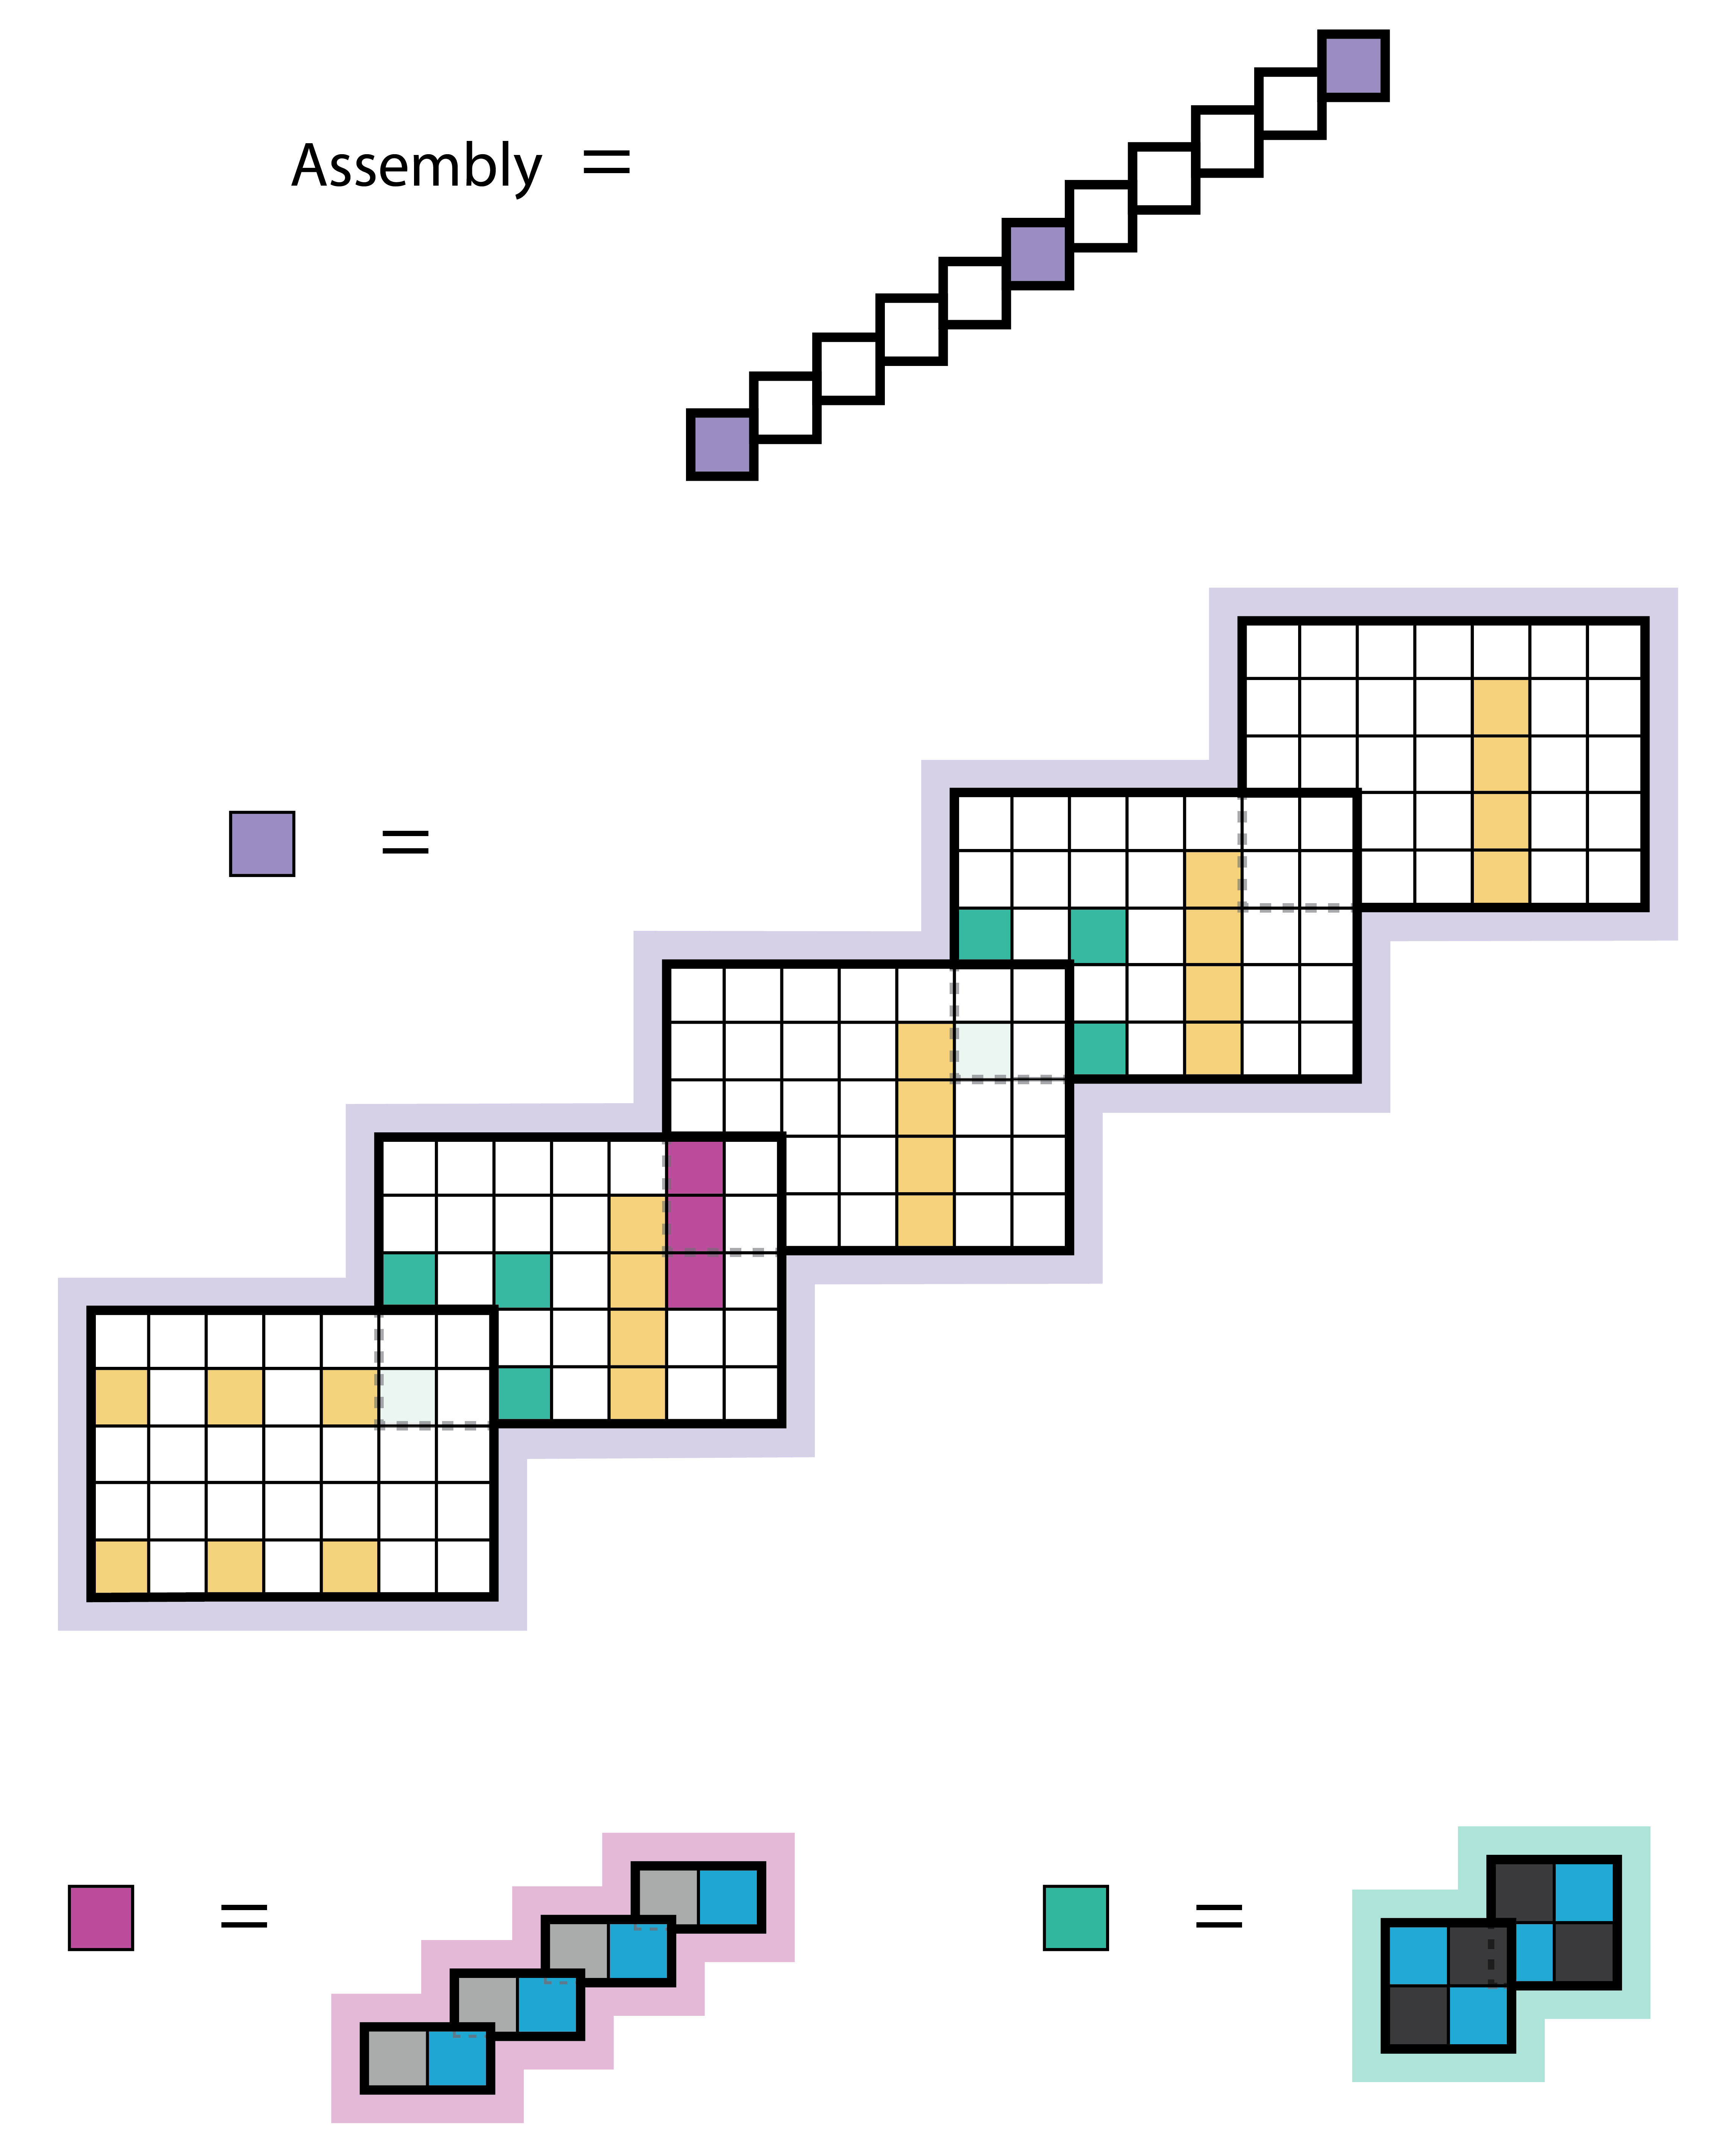
\includegraphics[width=\linewidth]{HierDataStructure.png}
  \caption{Sparse, hierarchical data structure behind the lattice assembly shown in Figure \ref{fig:CompositeCells}.  White squares indicate null elements.  The full lattice assembly is stored in an 11x1x1 array with only three non-null elements, shown at the top. Within each purple cell (composite cell 3) is a 5x7x5 cell definition, containing two more types of composite cells and one non-composite cell type.  Composite cell 2 (bottom left) contains a 4x2x1 cell array and composite cell 1 (bottom right) contains a 2x2x2 cell array, both filled with non-composite cell types.}
  \label{fig:HierDataStructure}
\end{figure}

The hierarchical data structure used in DMDesign is depicted graphically in Figure \ref{fig:HierDataStructure}.  In this structure, cells are stored in a minimally-sized 3D array whose upper and lower bounds change as the bounds of the assembly grow and shrink.  Each composite cell type has a definition that includes its own 3D array of cells.  This structure allows for a potentially very concise description of assemblies with many regions of self-similarity.  In order to render an assembly to the screen, a lattice data structure must be parsed recursively until all composite definitions have been fully evaluated down to their lowest level of description.\\

Along with a concise design description, hierarchy offers other advantages.  Changes to a composite cell definition propagate out to all the instances of that composite cell within an assembly, including instances contained within any parent composite cell definitions.  This means users can rapidly design large assemblies of cells and achieve some basic parametric control over their composition.    Hierarchical delineations often correspond to behavioral compartmentalization within a design.  Though not yet explored in this work, it would be interesting to leverage hierarchical design structure in simulation.\\

\begin{figure}
  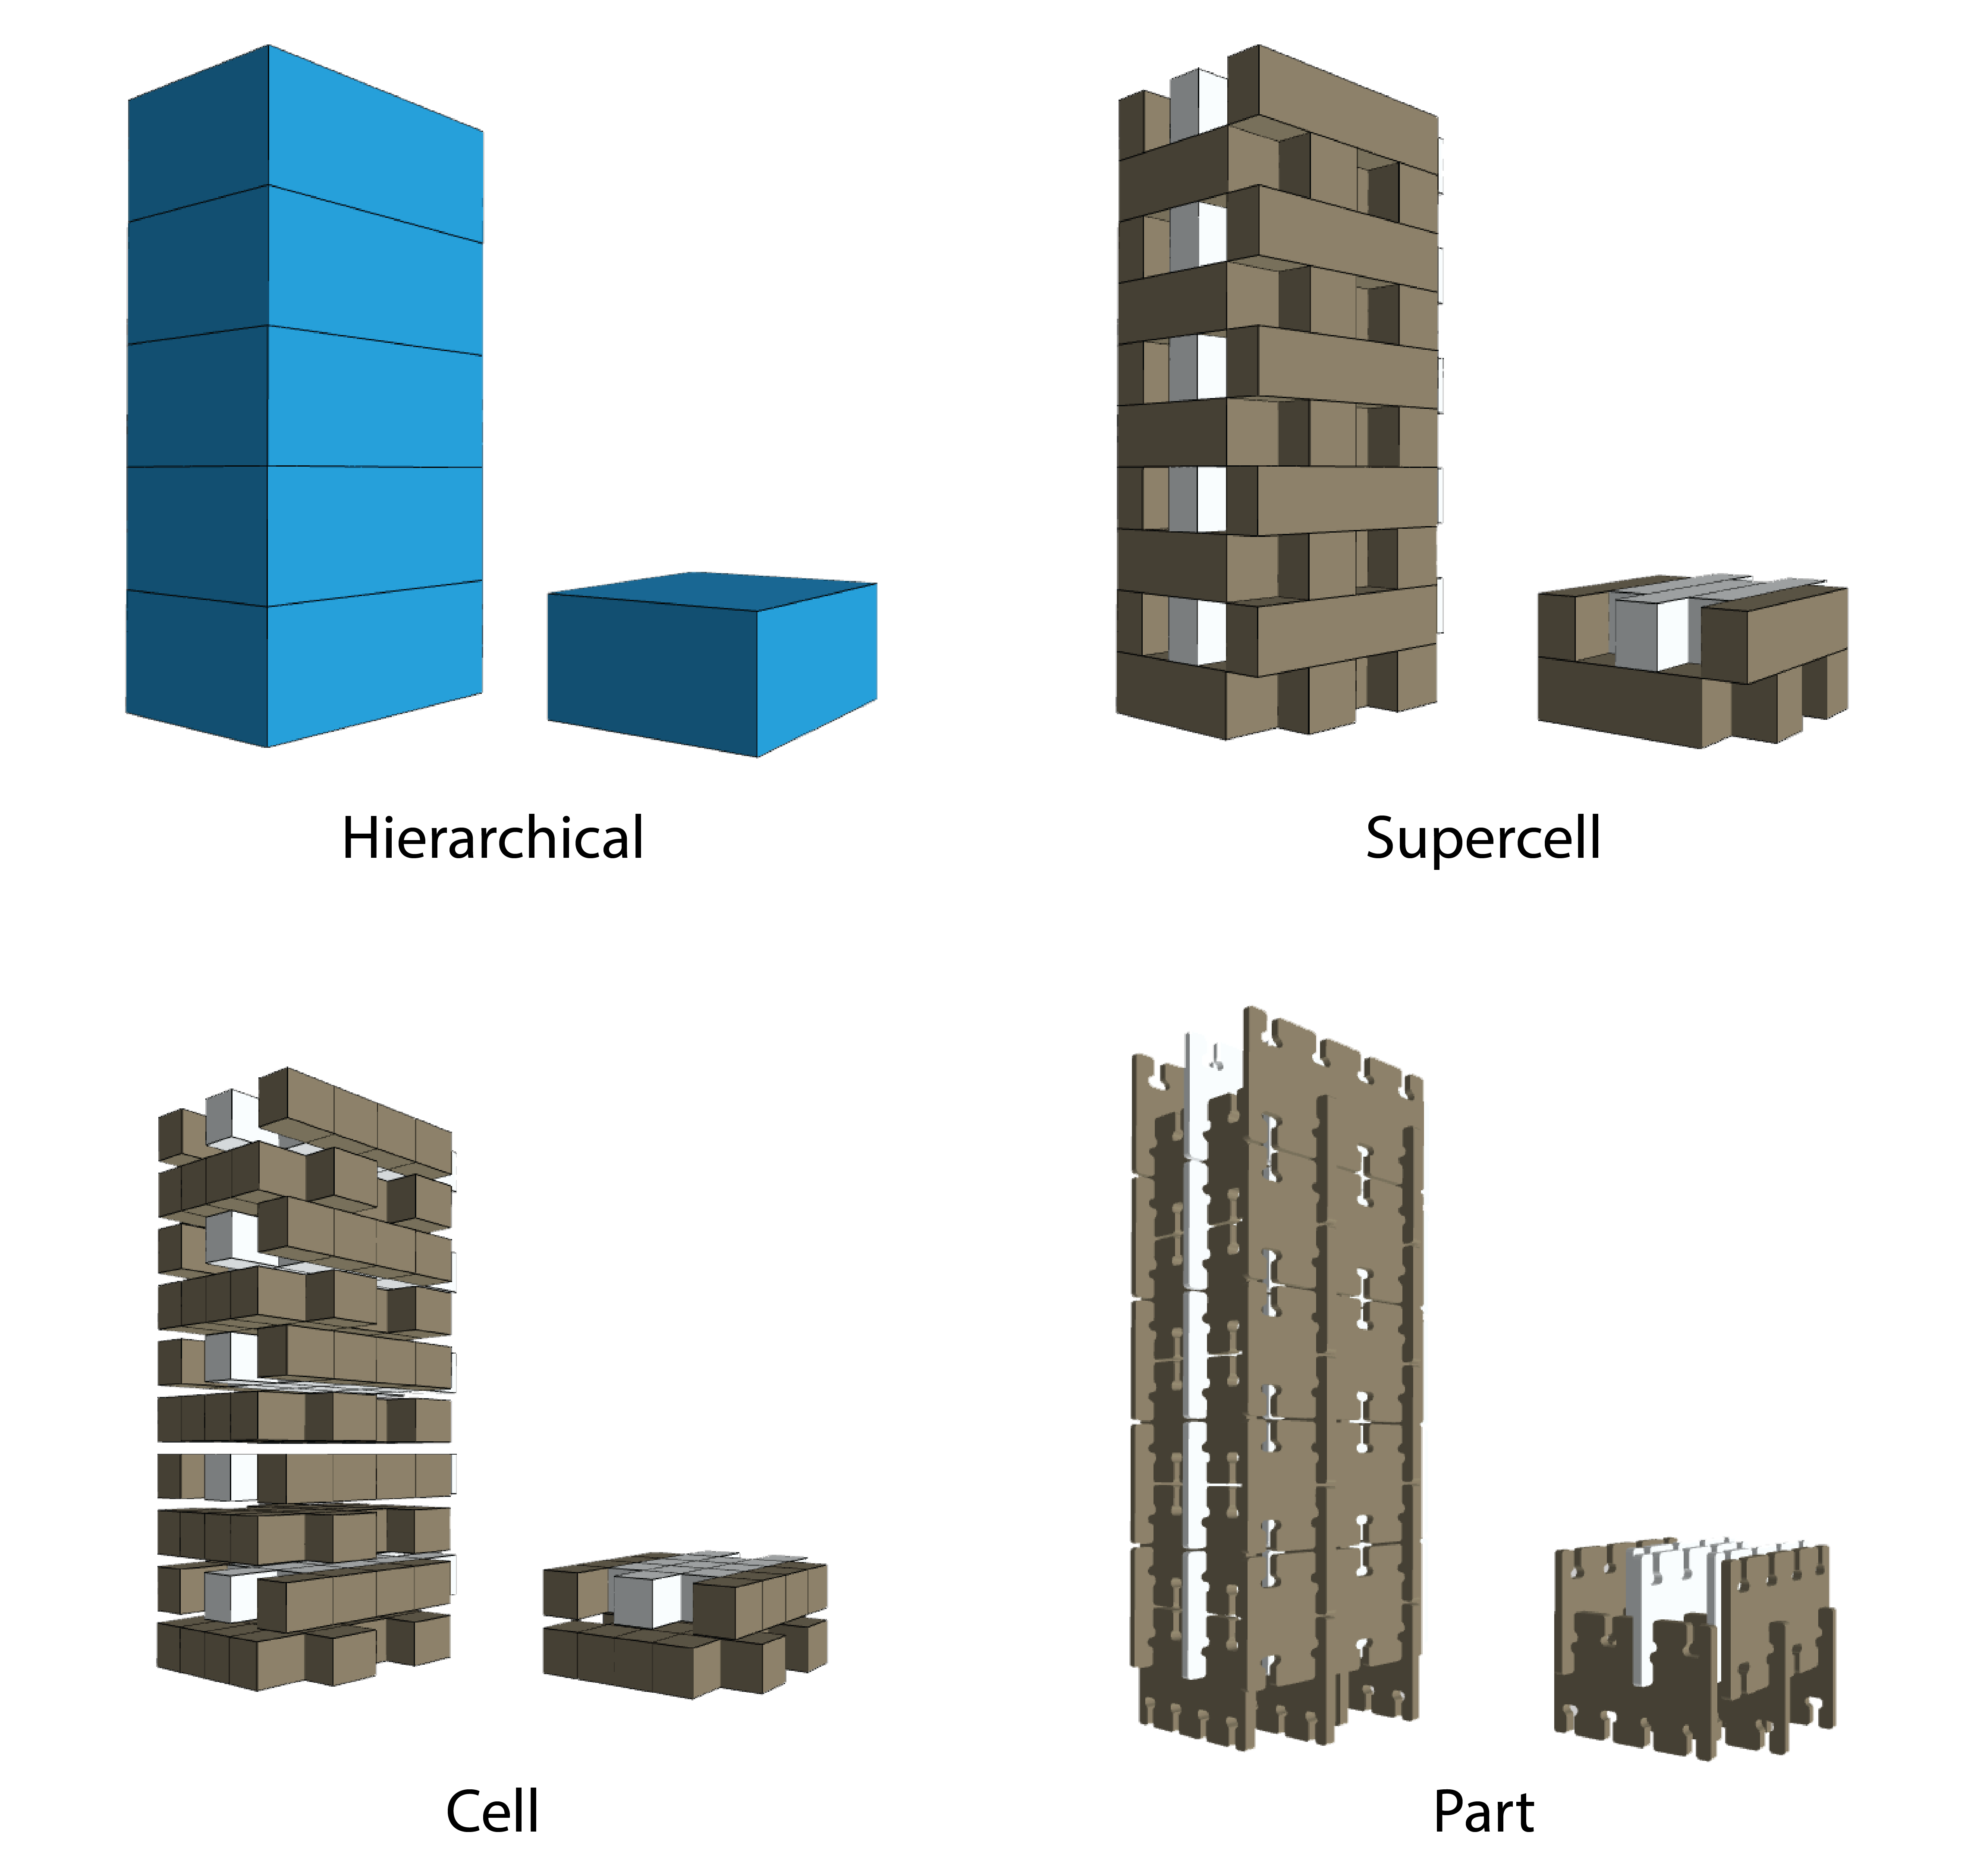
\includegraphics[width=\linewidth]{HierarchyGik.png}
  \caption{Four views of the same capacitive assembly of a GIK Lattice.  Nine conducting and insulating GIK parts are arranged to form a capacitive unit structure.  A composite cell consisting of this capacitive unit pattern is stacked vertically five times to form a larger capacitive tower.  Top left shows the individual composite cells in blue, top right shows the composite cells broken down into their constituent supercells.  Each GIK supercell is made from four cells in a cubic lattice, this deconstruction is visualized at the cell level (bottom left).  Finally, the underlying physical geometry of the assembly is depicted in the bottom right.  Lattices in which the physical part is wholly contained within unit cell do not have the supercell layer of description.}
  \label{fig:HierarchyGik}
\end{figure}

Under certain circumstances, hierarchy manifests itself in one more way.  For some applications, the physical part being represented is not contained wholly within a single cell object.  For example, in a GIK lattice, one GIK part is made from four cells on a cubic lattice.  In order to enforce valid GIK designs and allow the user to control the grouping of cells on the lattice into GIK parts, cells are organized into a mid-level hierarchical structure called a "supercell" (Figure \ref{fig:HierarchyGik}).  These supercells are the lowest level object that can be placed in the GIK design workflow.  Applications for which one cell represents one physical part or a collection of parts do not have the supercell delineation.

\section{Assembler Abstraction}

\begin{figure}
  \includegraphics[width=\linewidth]{machineabstraction.png}
  \caption{Three assembly processes controlled by DMDesign.  Top shows assembly of octahedron voxels in an edge-connected octa lattice by the "Batmen" assembler by Ben Jenett and Matt Carney.  Middle shows assembly of the same octahedron voxels by a 3-axis shopbot with custon end-effector designed by Ben Jenett.  Bottom show assembly of conducting and insulation GIK parts in a cubic lattice by the "Stapler" assembler by Will Langford.  \textit{Image Credit: (top left) Matt Carney 2015 and (bottom left) Will Langford 2015}}
  \label{fig:machineabstraction}
\end{figure}

Due to the variety of lattice configurations and assembly strategies, I've organized the CAM workflow of DMDesign so that users can construct a diversity of machine configurations through a simple interface using a few modular, abstract classes.  In addition to general machine configuration, global CAM variables, including lattice pitch, machine origin, clearances, and feed rates are all accessible through DMDesign (Figure \ref{fig:CAMmachineglobals}).  Once a user has dialed in their settings, a "stock simulation" of the assembly process may be visualized within the software, showing a complete run through of all g-code or other machine commands with a side by side 3D visualization of the assembler.  Finally, using a nodeJS interface, machine commands can be sent directly from DMDesign to the assembler.\\

At the time of writing this, three different machines have been used to assemble parts through DMDesign, depicted in Figure \ref{fig:machineabstraction}.  The "Batmen" assembler (its name deriving from a portmanteau of its creators - Ben Jenett and Matt Carney) is a 3-axis XYZ gantry with locking feet that locomotes across a lattice while placing octahedron voxels.  It is driven by a TinyG controller \cite{Synthetos2016} and consumes standard g-code commands.  The Shopbot is a 3-axis XYZ gantry with a custom end effector designed by Ben Jenett to pick and place the same octahedron voxels as Batmen.  The Shopbot runs off a simplified g-code-like protocol called shopbot protocol (OpenSBP) \cite{Shopbot2016}.  The "Stapler" assembler, designed by Will Langford, is a 4-axis XYZ gantry with a rotary stage that assembles GIK electronic components in an alternating "lego" configuration on a cubic lattice.  Like Batmen, the Stapler runs off a TinyG controller.  Many more machine configurations are theoretically supported by DMDesign.\\

\begin{figure}
  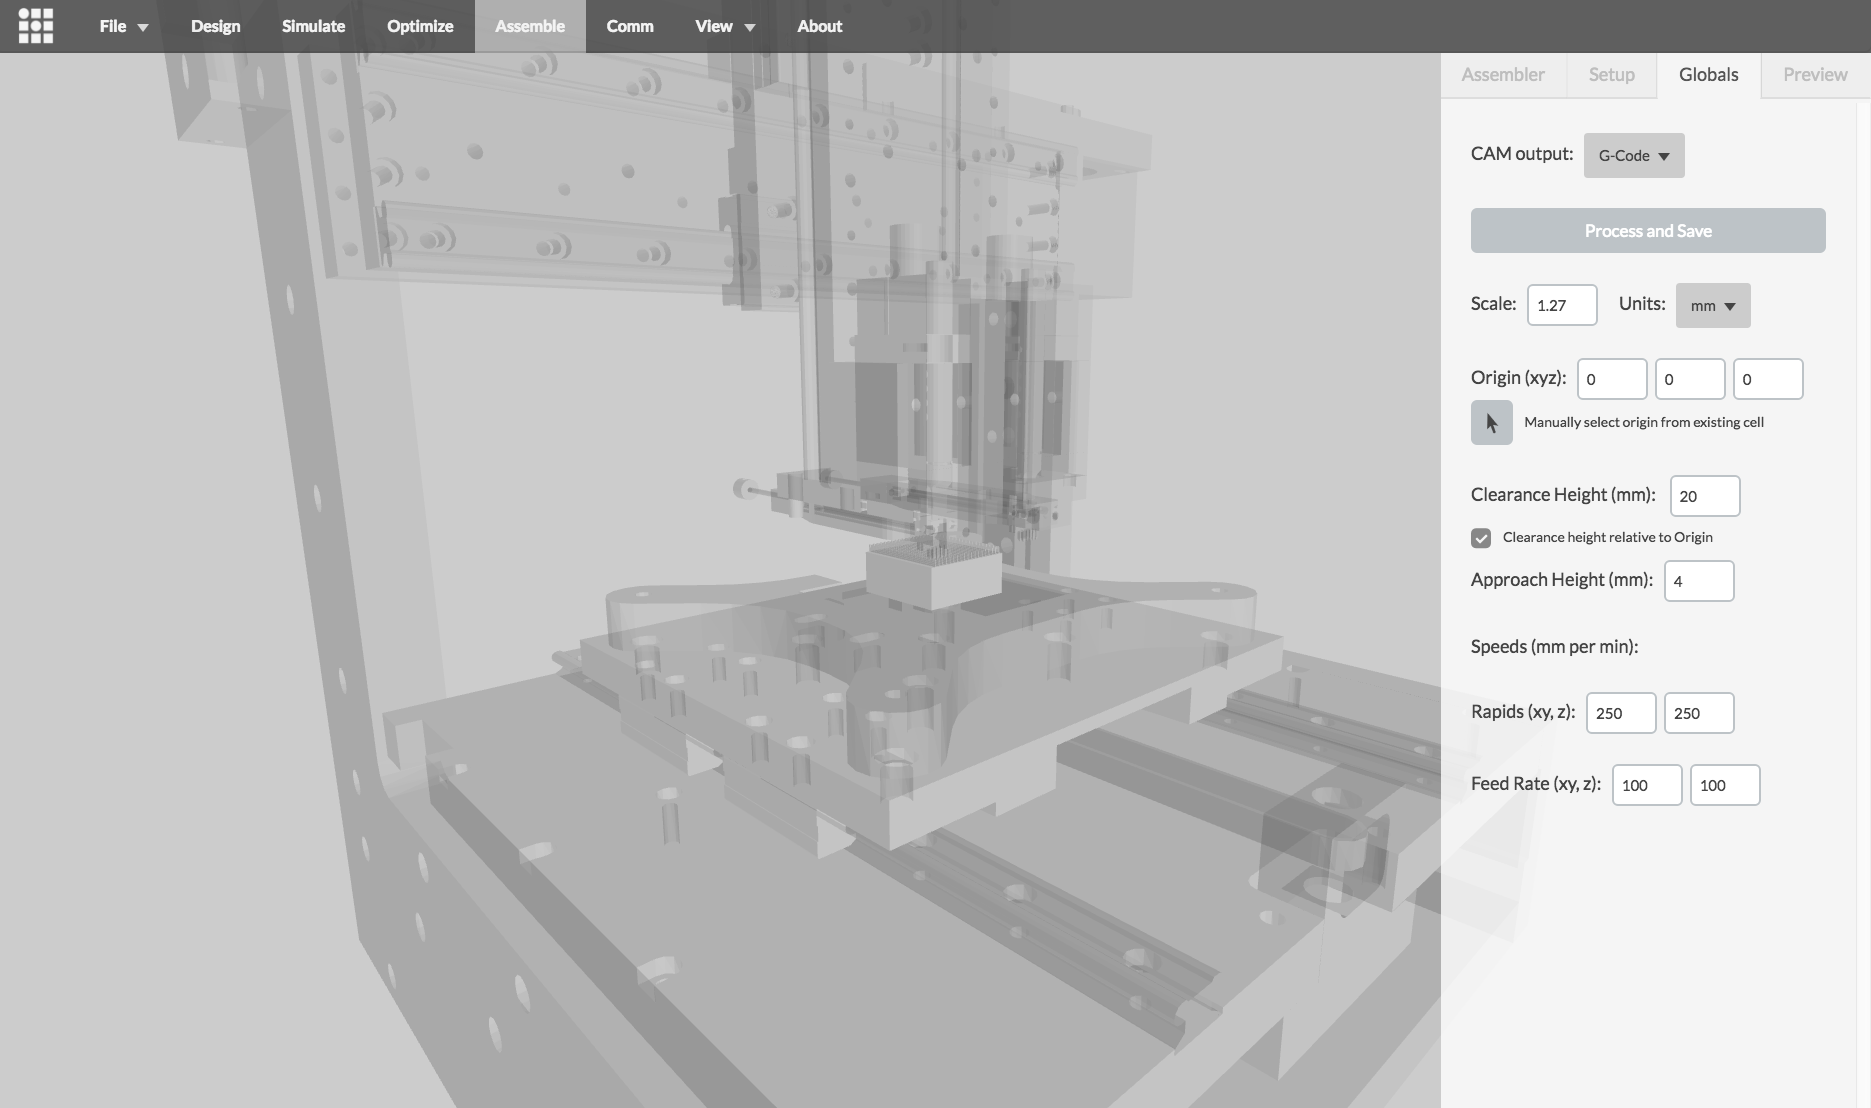
\includegraphics[width=\linewidth]{CAMmachineglobals.png}
  \caption{Interface for defining global assembly variables such as lattice pitch, machine origin, clearances, and feed rates.}
  \label{fig:CAMmachineglobals}
\end{figure}

\begin{figure}
  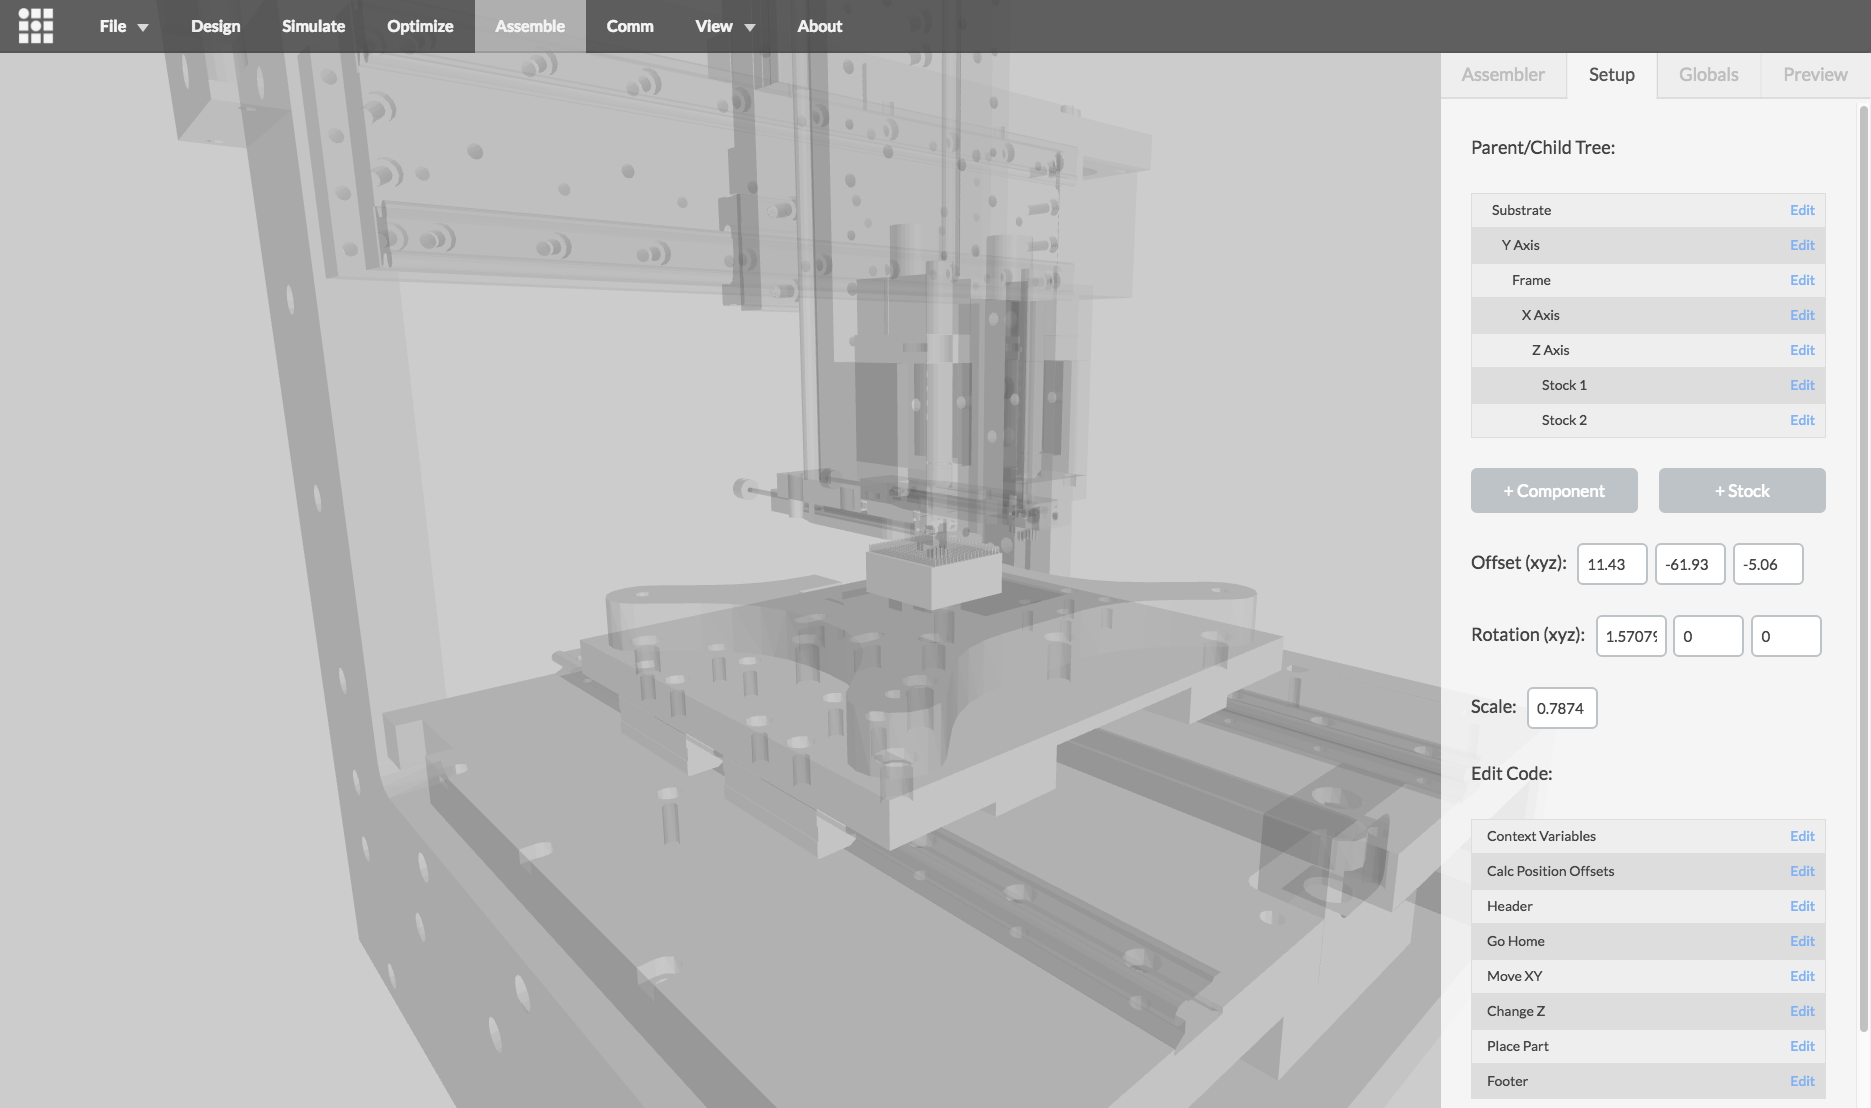
\includegraphics[width=\linewidth]{CAMmachinesetup.png}
  \caption{Machine configuration interface allows users to edit and save their own custom machine configuration files.  Using a format similar to the Universal Robot Description Format, machine kinematics and constraints are described by a series of links and joints connected to each other through parent/child relationships.  The parameters of the machine description are used to calculate inverse kinematics.}
  \label{fig:CAMmachinesetup}
\end{figure}

\begin{figure}
  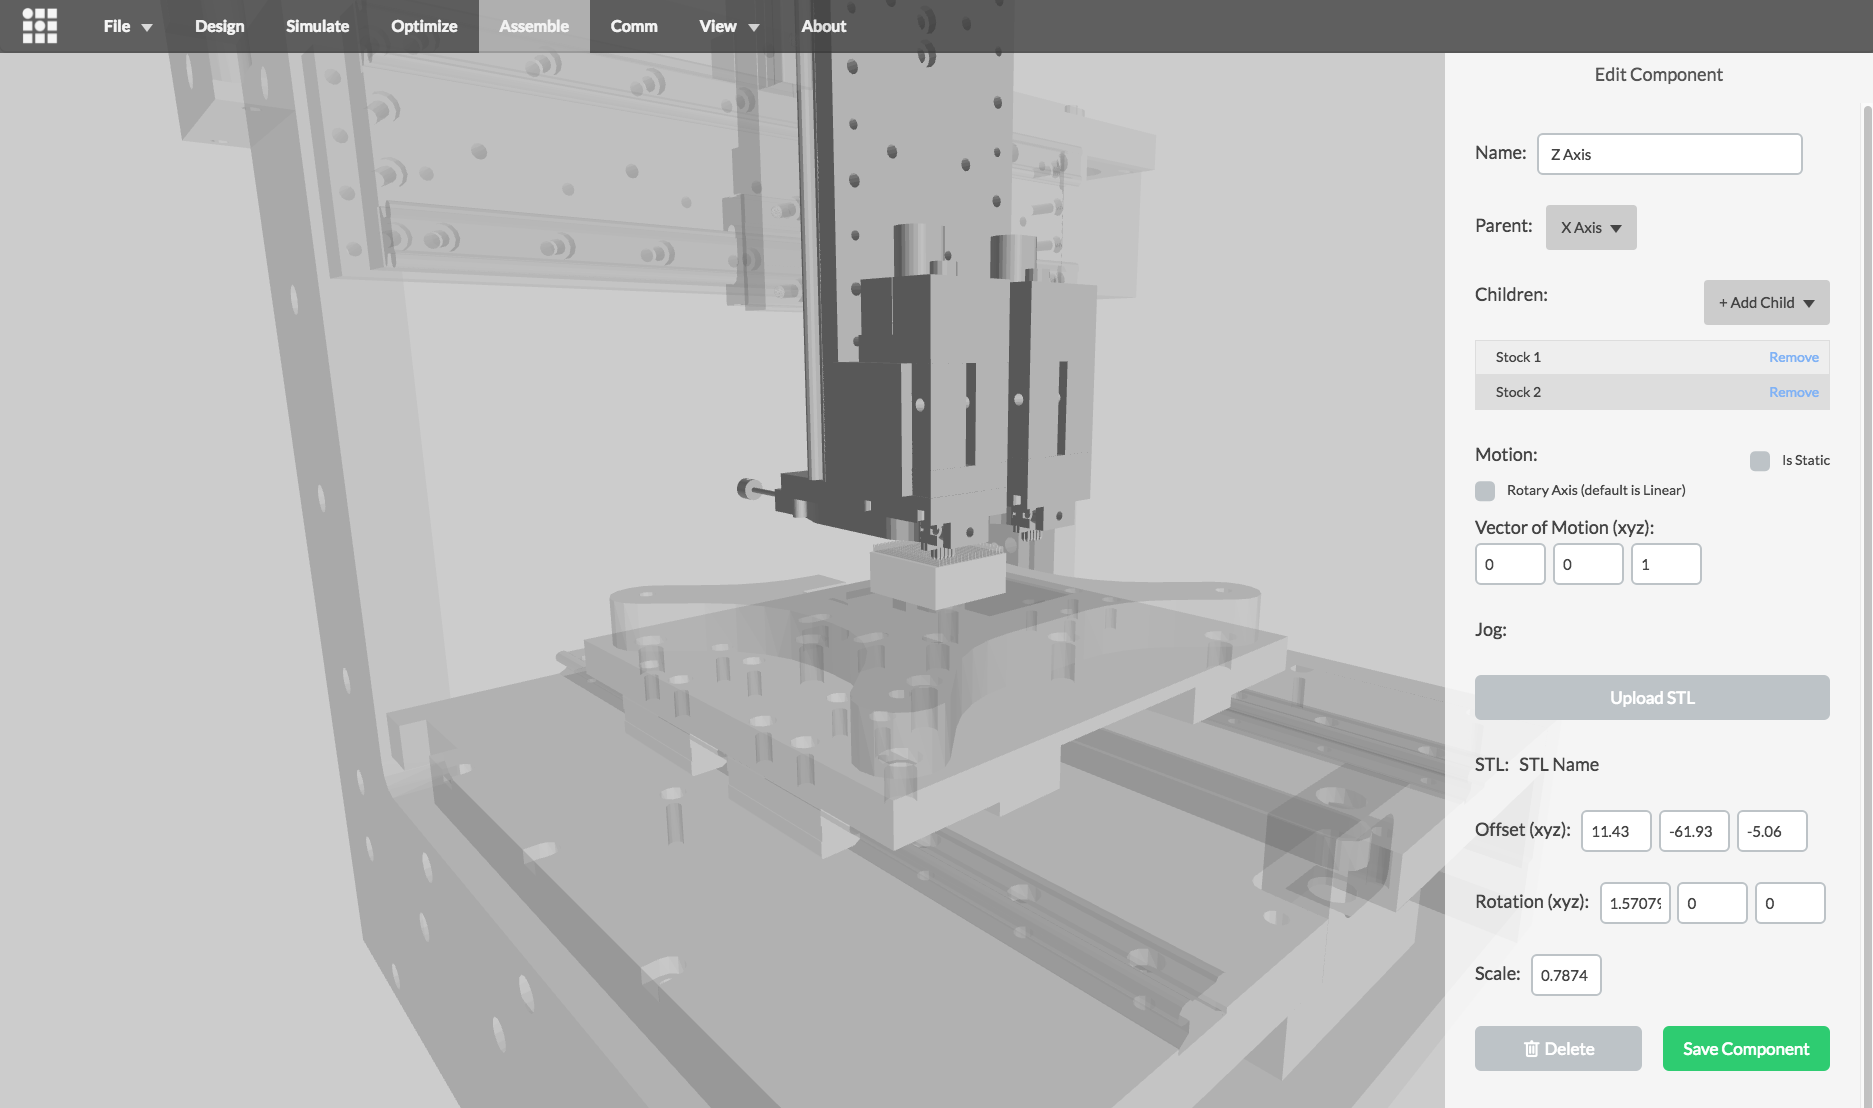
\includegraphics[width=\linewidth]{CAMbodydetail.png}
  \caption{Another view of the machine configuration interface shows a detail view of the setup for the "Stapler" assembler z-axis.}
  \label{fig:CAMbodydetail}
\end{figure}

Custom machine configurations are stored in a compact JSON format based on the Universal Robot Description Format (URDF) \cite{ROS2016}.  In this description, "links" and "joints" are connected to each other through parent/child relationships (Figure \ref{fig:CAMmachinesetup}).  Links are the rigid bodies in a machine; each link contains information about its kinematic properties and any meshes that might be associated with it (Figure \ref{fig:CAMbodydetail}).  Joints describe the constraints that govern the motion between two links and the range of motion available.  From this information, the inverse kinematics of the machine can be calculated and used to generate a valid path planning strategy.\\

\begin{figure}
  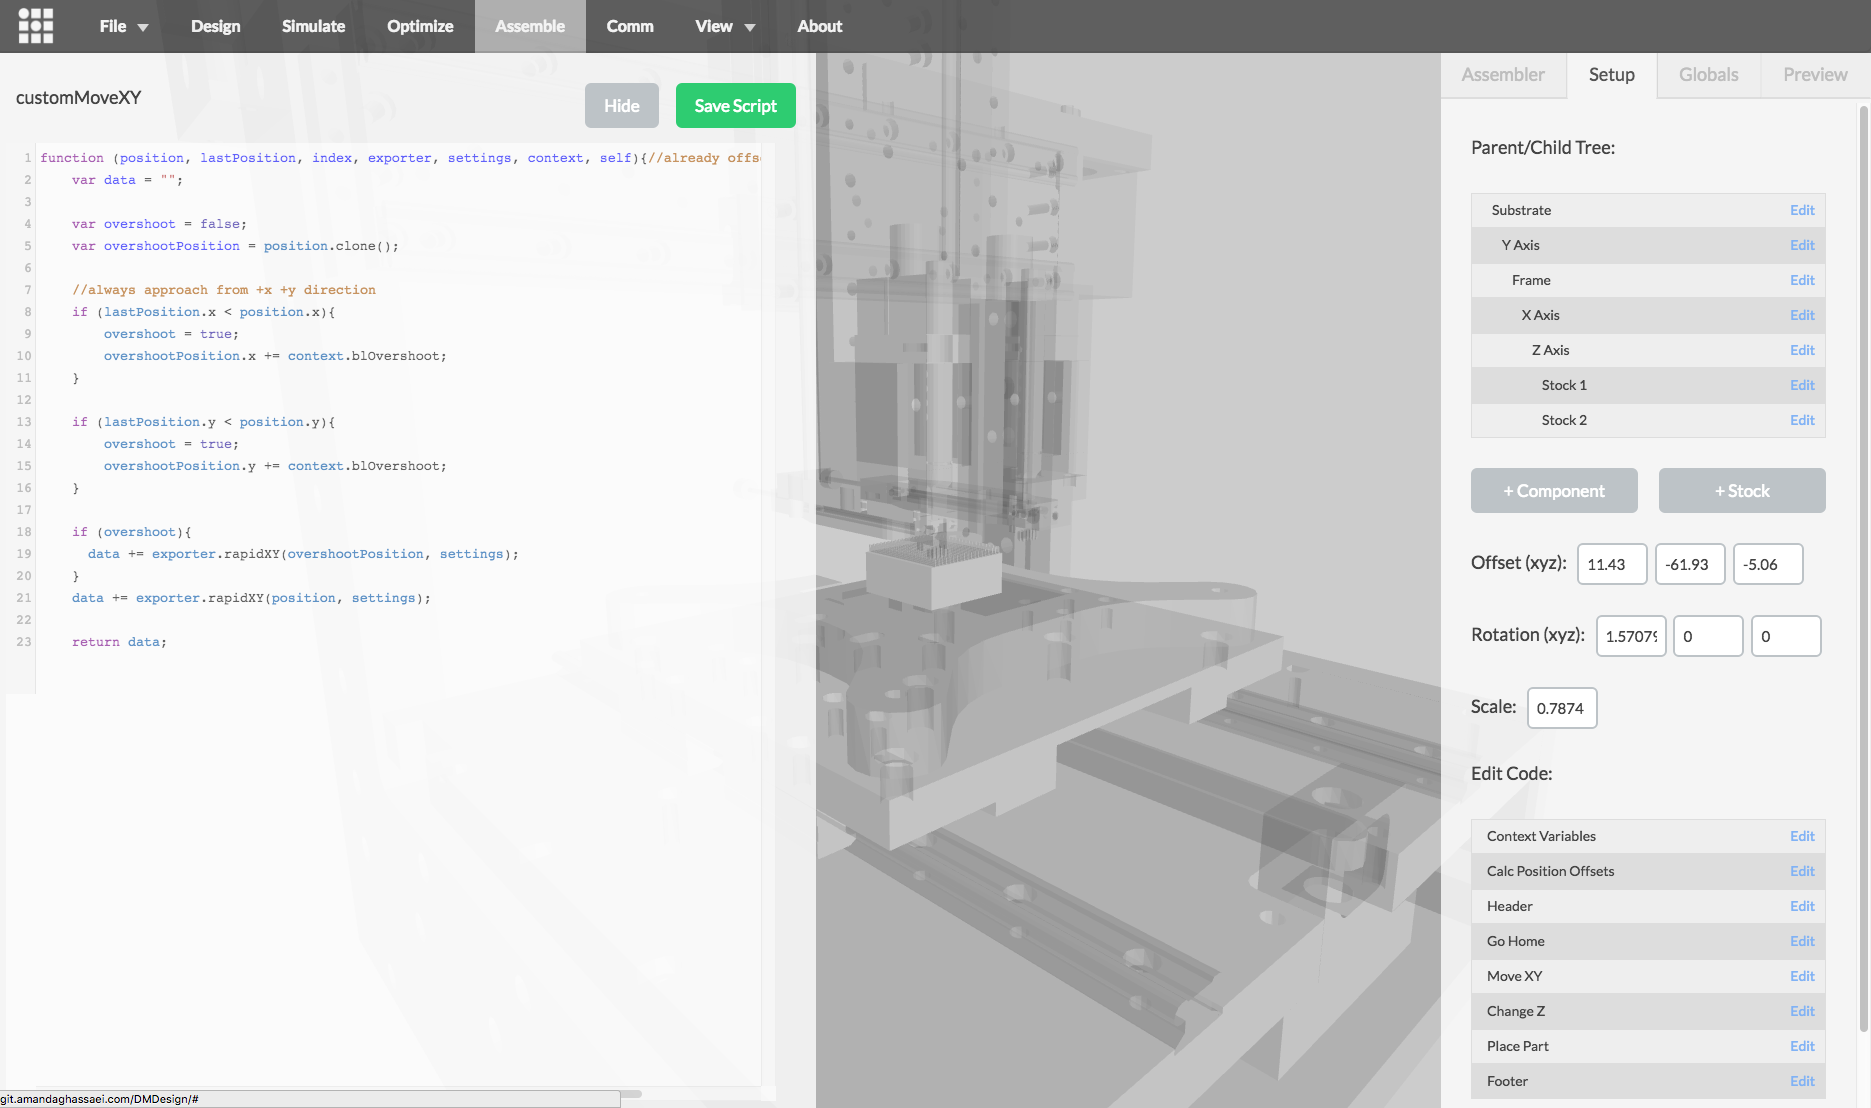
\includegraphics[width=\linewidth]{CAMcustomCode.png}
  \caption{Scripting interface for custom machine configuration.  This screenshot shows a user-defined function that calculates XY traversals with added backlash compensation specific to the "Stapler" assembler.  Other user-defined functions are listed in the bottom right, including: context variables, header, place part, footer, and others.}
  \label{fig:CAMcustomCode}
\end{figure}

Unique machine configurations often require special control logic to address the idiosyncrasies of a particular assembly process.  In order to accommodate a wide variety of potential machine configurations (and give more power to the end user) I've created a set of user-definable functions that can be edited and saved within DMDesign.  Users can define their own environmental variables and construct custom functions to handle traversals, picking up and placing parts, and headers and footers.  Within each of these functions, information such as current part index, position, material type, and any user-defined variables are available.  To date, this feature has been used for backlash compensation and multimaterial head placement of the "Stapler" assembler.  Eventually, this capability could grow to support closed-loop control between the machine and DMDesign for on-the-fly path planning or error correction.\\

\section{Off-Ramps}

\begin{figure}
  \includegraphics[width=\linewidth]{Brickset.png}
  \caption{SEM image of GIK assembly fabricated on a \href{http://www.nanoscribe.de/en/products/photonic-professional-gt/}{Nanoscribe Photonic Professional GT} using a technique called "two-photon lithography" to a resolution of 150nm.  Designed in DMDesign, geometry exported as STL mesh.  \textit{Image Credit: Prashant Patil 2015}}
  \label{fig:BrickSet}
\end{figure}

The intention behind DMDesign is not to replace all existing design and manufacturing workflows, but rather, to create an environment that better accommodates and, at times, leverages the discrete construction of digital materials.  In some cases, users will want to interface between DMDesign and other CAD, simulation, and CAM processes.\\

Currently, DMDesign supports \href{https://en.wikipedia.org/wiki/STL_(file_format)}{STL} export of assembly geometries.  Users can export geometry by material, and choose between the abstracted cell meshes or the more detailed part geometry.  These STLs have been used in 3D printing workflows, included nano-3D-printing (Figure \ref{fig:BrickSet}), photorealistic rendering in \href{https://www.blender.org/}{Blender}, and as reference geometry for simulations in \href{https://www.comsol.com/}{COMSOL}.

}
